
\chapter{Vectors in Three Dimensions}

Fundamentally, vectors are mathematical objects that we can add together and take multiples of, in both cases obtaining another vector. We will consider vectors in a general setting later on, but in this chapter we will consider vectors in $\R^3$, three dimensional space. Specifically, we will take a geometric approach, thinking of vectors as position vectors and using Euclidean notions of points, lines, planes, etc.

We begin by choosing a point $O$ as the origin. Then points $A$ and $B$ have position vectors
$$
\vv{a} = \overrightarrow{OA}, \quad\quad \vv{b} = \overrightarrow{OB}.
$$

\begin{center}
	\begin{tikzpicture}
	\coordinate (origin) at (0,0);
	\coordinate (a) at (4, 0.25);
	\coordinate (b) at (1.5, 2.25);

	\draw (origin) node [anchor=north east] {$O$};

	\draw [->,>=stealth] (origin) -- (a) node [anchor=north west] {$A$} node [pos=0.6, anchor=north] {$\vv{a}$};
	\draw [->,>=stealth] (origin) -- (b) node [anchor=north west] {$B$} node [pos=0.6, anchor=north west] {$\vv{b}$};
	\end{tikzpicture}
\end{center}

The vectors have length $|\vv{a}| = |\overrightarrow{OA}|$, the distance between $O$ and $A$. We also let $\vv{0}$ denote the position vector of $O$.

\section{Vector Addition and Scalar Multiplication}

The most important operations on vectors (in $\R^3$ and in general) is vector addition and scalar multiplication. We define these geometrically as follows.

\begin{definition}[Scalar Multiplication in $\R^3$]
	GIven $\vv{a}$, the position vector for a point $A$, and a scalar $\lambda \in \R$, we define \vocab{scalar multiplication} $\lambda \vv{a}$ to be the position vector for the point $A'$ on the line $OA$ such that
	$$
	|\lambda \vv{a} | = |OA'| = |\lambda| |\vv{a}|,
	$$
	with the vector being in the direction $\overrightarrow{OA}$ if $\lambda$ is positive, and in the opposite direction otherwise.
\end{definition}

\begin{center}
	\begin{tikzpicture}
	\coordinate (origin) at (0,0);
	\coordinate (a) at (2, 0.17);

	\draw (origin) node [anchor=north east] {$O$};

	\draw [->,>=stealth, dashed] ($(origin)  - (a) - (a)$) -- ($(a) + (a) + (a) + (a) $);

	\draw [->,>=stealth, color=blue] (origin) -- ($(a) + (a) + (a)$) node [anchor=north west, color=black] {$A'$} node [pos=0.8, anchor=north] {$\lambda\vv{a}$};
	\draw [->,>=stealth, color=black] (origin) -- ($(a)$) node [anchor=north west, color=black] {$A$} node [pos=0.6, anchor=north, color=black] {$\vv{a}$};
	
	\end{tikzpicture}
\end{center}

If two vectors are scalar multiples of each other, then we say that they are \vocab{parallel}. Specifically, we write $\vv{a} \parallel \vv{b}$ if and only if $\vv{a} = \lambda \vv{b}$ or $\vv{b} = \lambda \vv{a}$ for some $\lambda \in \R$. Notably, $\vv{a} \parallel \vv{0}$ for all vectors $\vv{a}$.


\begin{definition}[Vector Addition in $\R^3$]
	Given $\vv{a}$ and $\vv{b}$, position vectors of points $A$ and $B$, if $\vv{a} \not \parallel \vv{b}$, we construct the parallelogram $OACB$, and define \vocab{vector addition} $\vv{a} + \vv{b} = \vv{c}$. 
\end{definition}


\begin{center}
	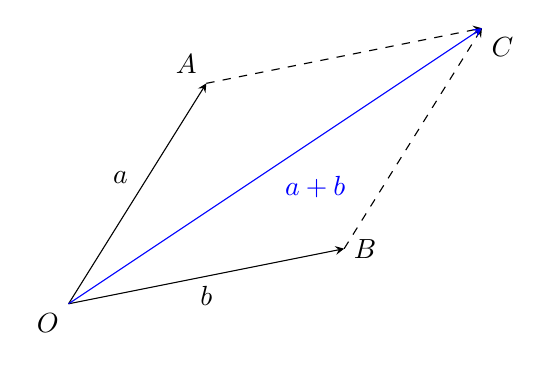
\begin{tikzpicture}[xscale=1.4, yscale=1.4]
	\draw (0, 0) node [anchor=north east] {$O$};
	\draw [->,>=stealth] (0, 0) -- (2.5, 0.5) node [anchor=west] {$B$} node [pos=0.5, anchor=north] {$\vv{b}$};
	\draw [->,>=stealth] (0, 0) -- (1.25, 2.0) node [anchor=south east] {$A$} node [pos=0.5, anchor=south east] {$\vv{a}$};
	\draw [->,>=stealth, dashed] (1.25, 2.0) -- (3.75, 2.5);
	\draw [->,>=stealth, dashed] (2.5, 0.5) -- (3.75, 2.5);
	\draw [->,>=stealth, color=blue] (0,0) -- (3.75, 2.5) node [pos=0.5, anchor=north west] {$\vv{a} + \vv{b}$};
	\draw (3.75, 2.5) node [anchor=north west] {$C$};
	\end{tikzpicture}
  \end{center}

If $\vv{a} \parallel \vv{b}$, then writing $\vv{a} = \alpha \vv{u}$ and $\vv{b} = \beta \vv{u}$ where $\vv{u}$ is a unit vector, then $\vv{a} + \vv{b} = (\alpha+ \beta) \vv{u}$.

Given some set of vectors $\vv{v_1}$, $\vv{v_2}$, $\dots$, $\vv{v_k}$, we can form a \vocab{linear combination}
$$
\lambda_1 \vv{v_1} + \lambda_2 \vv{v_2}  + \cdots + \lambda_k \vv{v_k},
$$
where $\lambda_i \in \R$. With this in mind, we can consider the set of all vectors that can be formed as a linear combination of some vectors.

\begin{definition}[Span]
	For vectors $\vv{v_1}$, $\vv{v_2}$, $\dots$, $\vv{v_k}$, we define their \vocab{span} to be the set
	$$
	\vecspan\{\vv{v_1}, \vv{v_2}, \dots, \vv{v_k} \} = \{ \lambda_1 \vv{v_1} + \lambda_2 \vv{v_2}  + \cdots + \lambda_k \vv{v_k} \mid \lambda_i \in \R \}.
	$$
\end{definition}

If two vectors $\vv{a} \not \parallel \vv{b}$, then $\vecspan\{\vv{a}, \vv{b}\}$ is a plane through $OAB$.

Vector addition and scalar multiplication obey some basic properties that you should keep in mind, as they will be used again when we define vectors in a general sense.

\begin{proposition}[Basic Properties of Vector Operations]
For any vectors $\vv{a}$, $\vv{b}$ and $\vv{c}$,
\begin{enumerate}[label=(\roman*)]
	\item Vectors along with vector addition form an abelian group.
	\item $\lambda(\vv{a} + \vv{b}) = \lambda \vv{a} + \lambda \vv{b}$.
	\item $(\lambda + \mu)\vv{a} = \lambda\vv{a} + \mu\vv{a}$.
	\item $\lambda(\mu \vv{a}) = (\lambda \mu) \vv{a}$.
\end{enumerate}
\end{proposition}
\begin{proof}[Proof Sketch]
	Check geometric definitions. Checking associativity of vector addition will require the construction of a parallelepiped.
\end{proof}


\section{The Dot Product}

We saw in the previous section how to add vectors, and how to multiply a vector by a scalar. In the next two sections, we will consider how to multiply a vector and a vector. 
We will first define the \emph{scalar} or \emph{dot product}.
Consider two vectors $\vv{a}$ and $\vv{b}$, with the angle between then being $\theta$ as shown.

\begin{center}
    \begin{tikzpicture}
        \coordinate (origin) at (0,0);
        \coordinate (z) at (1.75, 1.9);
        \coordinate (z1) at (3.25, 0);

        % \draw (0, 0) node [anchor=north east] {$O$};
        \draw [->,>=stealth] (0, 0) -- (z1) node [anchor=west] {$\vv{a}$};
        %  node [pos=0.5, anchor=north] {$\vv{a}$};
        \draw [->,>=stealth] (0, 0) -- (z) node [anchor=west] {$\vv{b}$};
        %  node [pos=0.5, anchor=south east] {$\vv{b}$};
        \pic [draw, ->, angle eccentricity=1.2, angle radius=1.25cm, color=purple] {angle = z1--origin--z};
        \draw (0.8, 0.38) node {$\theta$};
	\end{tikzpicture}
  \end{center}

\begin{definition}[Dot Product]
    For two vectors $\vv{a}$ and $\vv{b}$, and $\theta$ the angle between them as shown, we define the \vocab{scalar} or \vocab{dot product} as
    $$
    \vv{a} \cdot \vv{b} = |\vv{a}| |\vv{b}| \cos \theta.
    $$

    [Note that $\theta$ is defined unless $\vv{a}$ or $\vv{b}$ is zero, but then $|\vv{a}| = 0$ or $|\vv{b}| = 0$ and $\vv{a} \cdot \vv{b} = 0$.]
\end{definition}

The scalar product encodes an angle condition, and gives us a dot for perpendicularity. We say vectors $\vv{a}$ and $\vv{b}$ are \vocab{orthogonal} or \vocab{perpendicular} if and only if $\vv{a} \cdot \vv{b} = 0$. This corresponds with $\theta = \pm \pi/2$, or with either $|\vv{a}| = 0$ or $|\vv{b}| = 0$.

There is a geometric interpretation of the dot product. Fundamentally, the dot product is a \emph{projection}. For $\vv{a} \neq \vv{0}$, the quantity $|\vv{b}| \cos \theta$ is the component of $\vv{b}$ when projected along the direction of $\vv{a}$.

\begin{center}
    \begin{tikzpicture}
        \coordinate (origin) at (0,0);
        \coordinate (z) at (1.75, 1.9);
        \coordinate (z1) at (3.25, 0);

        \draw [dashed] (0, 0) -- (5.25, 0);

        \draw [color=blue, dashed] (z) -- (1.75, 0);

        \fill (1.75,0)  circle[color=blue, radius=1pt];

        % \draw (0, 0) node [anchor=north east] {$O$};
        \draw [->,>=stealth] (0, 0) -- (z1) node [anchor=north] {$\vv{a}$};
        %  node [pos=0.5, anchor=north] {$\vv{a}$};
        \draw [->,>=stealth] (0, 0) -- (z) node [anchor=west] {$\vv{b}$};
        %  node [pos=0.5, anchor=south east] {$\vv{b}$};
        \pic [draw, ->, angle eccentricity=1.2, angle radius=0.8cm, color=purple] {angle = z1--origin--z};
        \draw (0.533333333, 0.253333333) node {\small $\theta$};

        % \draw (1.75, 0) node [anchor=north] {$\vv{b}_{\parallel}$};
        \draw [color=blue] (0,0) -- (1.75, 0);

        \draw [decoration={brace, mirror, raise=0.4cm}, decorate] (0,0) -- (1.75, 0) node [pos=0.5, anchor=north, yshift=-0.45cm] {\footnotesize $|\vv{b}| \cos \theta$};
        \draw [densely dashed] (0,0) -- (0, -0.4cm);
        \draw [densely dashed] (1.75,0) -- (1.75, -0.4cm);
	\end{tikzpicture}
  \end{center}

  \begin{proposition}[Basic Properties of the Dot Product]
      For any vectors $\vv{a}$ and $\vv{b}$,
      \begin{enumerate}[label=(\roman*)]
          \item $\vv{a} \cdot \vv{b} = \vv{b} \cdot \vv{a}$.
          \item $\vv{a} \cdot \vv{a} = |a|^2 \geq$, and $\vv{a} \cdot \vv{a} = 0$ if and only if $\vv{a} = \vv{0}$.
          \item $(\lambda \vv{a}) \cdot \vv{b} = \lambda (\vv{a} \cdot \vv{b}) = \vv{a} \cdot (\lambda \vv{b})$.
          \item $\vv{a} \cdot (\vv{b} + \vv{c}) = \vv{a} \cdot \vv{b} + \vv{a} \cdot \vv{c}$. 
      \end{enumerate}
  \end{proposition}
  \begin{proof}
      Properties (i) to (iii) follow directly from the definition of the dot product. Property (iv) follows from the geometric interpretation of the dot product shown above. 
  \end{proof}



\section{The Cross Product}

The next operation only works with vectors in three dimensions, and is the \emph{vector} or \emph{cross product}. As before, consider two vectors $\vv{a}$ and $\vv{b}$, and let $\theta$ be measured as shown with respect to $\hat{\vv{n}}$, a unit normal to the plane spanned by $\vv{a}$ and $\vv{b}$.

\begin{center}
    \begin{tikzpicture}
        \coordinate (origin) at (0,0);
        \coordinate (z) at (2.5, 0.6);
        \coordinate (z1) at (3.25, -0.35);

        % \draw (0, 0) node [anchor=north east] {$O$};
        \draw [->,>=stealth] (0, 0) -- (z1) node [anchor=west] {$\vv{a}$};
        %  node [pos=0.5, anchor=north] {$\vv{a}$};
        \draw [->,>=stealth] (0, 0) -- (z) node [anchor=west] {$\vv{b}$};
        %  node [pos=0.5, anchor=south east] {$\vv{b}$};
        \pic [draw, ->, angle eccentricity=1.8, angle radius=1.45cm, color=purple] {angle = z1--origin--z};
        
        \draw (1, 0.08) node {$\theta$};

        \draw [->,>=stealth, color=blue] (0,0) -- (0, 1.5) node [anchor=south] {$\hat{\vv{n}}$};
	\end{tikzpicture}
  \end{center}

  \begin{definition}[Cross Product]
For two vectors $\vv{a}$ and $\vv{b}$ with angle  $\theta$ measured as shown, we define the \vocab{vector} or \vocab{cross product} as
$$
\vv{a} \times \vv{b} = | \vv{a}| |\vv{b}| \sin \theta \hat{\vv{n}},
$$
where $\hat{\vv{n}}$ is a unit vector perpendicular to the plane spanned by $\vv{a}$ and $\vv{b}$.

[$\hat{\vv{n}}$ is defined up to a sign if $\vv{a} \not \parallel \vv{b}$, but changing the sign changes $\theta$ to $2\pi - \theta$, and thus leaves $\vv{a} \times \vv{b}$ unchanged. When $\hat{\vv{n}}$ is not defined ($\vv{a} \parallel \vv{b}$ or $\theta$ not defined), $\vv{a} \times \vv{b} = \vv{0}$.] 
  \end{definition}

  The geometric interpretation of the cross product is that $|\vv{a} \times \vv{b}|$ is the area of the parallelogram as shown.

  \begin{center}
    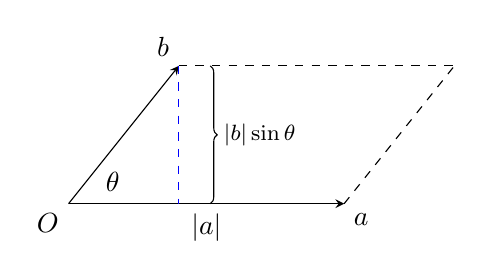
\begin{tikzpicture}[xscale=1.4, yscale=1.4]
    \draw (0, 0) node [anchor=north east] {$O$};
    
    \draw [->,>=stealth] (0, 0) -- (2.5, 0) node [anchor=north west] {$\vv{a}$} node [pos=0.5, anchor=north] {$|\vv{a}|$};
    \draw [->,>=stealth] (0, 0) -- (1, 1.25) node [anchor=south east] {$\vv{b}$};

    \draw (0.4, 0.2) node {$\theta$};

    \draw [dashed] (1, 1.25) -- (3.5, 1.25);
    \draw [dashed] (2.5, 0) -- (3.5, 1.25);

    \draw [dashed, color=blue] (1,1.25) -- (1, 0);
    \draw [decoration={brace, raise=0.4cm}, decorate] (1, 1.25) -- (1, 0) node [pos=0.5, anchor=west, xshift=0.45cm] {\footnotesize $|\vv{b}| \sin \theta$};
    
	% \draw [->,>=stealth, dashed] (1.25, 2.0) -- (3.75, 2.5);
	% \draw [->,>=stealth, dashed] (2.5, 0.5) -- (3.75, 2.5);
	% \draw [->,>=stealth, color=blue] (0,0) -- (3.75, 2.5) node [pos=0.5, anchor=north west] {$\vv{a} + \vv{b}$};
	% \draw (3.75, 2.5) node [anchor=north west] {$C$};
    \end{tikzpicture}
  \end{center}

  The direction of $\vv{a} \times \vv{b}$ gives the orientation of this parallelogram in space.   

For an alternate geometric interpretation, fix a vector $\vv{a}$ and consider some vector $\vv{x}$ with $\vv{x} \perp \vv{a}$. Then the transformation $\vv{x} \longmapsto \vv{a} \times \vv{x}$ corresponds with scaling $\vv{x}$ by $\vv{a}$ and rotating by $\pi/2$ in the plane perpendicular to $\vv{a}$.

\begin{proposition}[Basic Properties of the Cross Product]
    For vectors $\vv{a}$, $\vv{b}$ and $\vv{c}$,
    \begin{enumerate}[label=(\roman*)]
        \item $\vv{a} \times \vv{b} = - (\vv{b} \times \vv{a})$.
        \item $(\lambda \vv{a}) \times \vv{b} = \lambda (\vv{a}) \times \vv{b})$.
        \item $\vv{a} \times (\vv{b} + \vv{c}) = \vv{a} \times \vv{b} + \vv{a} \times \vv{c}$.
        \item $\vv{a} \times \vv{b} = \vv{0}$ if and only if $\vv{a} \perp \vv{b}$.
        \item $\vv{a} \times \vv{b} \perp \vv{a}, \vv{b}$, so $\vv{a} \cdot (\vv{a} \times \vv{b}) = \vv{b} \cdot (\vv{a} \times \vv{b}) = 0$. 
    \end{enumerate}
\end{proposition}
\begin{proof}[Proof Sketch]
    Check definitions.
\end{proof}

\section{Orthonormal Bases and Components}

So far we have considered vectors in a purely geometric sense. But just as a coordinate system can be used to reason about geometry, basis (and by extension components) can be used to reason about vectors. We will look at bases again in a more general setting later on, but for now we will focus on vectors in three dimensions.

When we use a cartesian coordinate system, we pick a set of axes and using them, we can describe the position of any point. In a similar way, a \emph{basis} is a set of vectors that span the space. That is, any vector can be written as a linear combination of vectors in the set. However we also have an additional requirement: this linear combination must be unique.

\begin{definition}[Basis -- Informal]
    We say that a set of vectors is a \vocab{basis} if any vector can be uniquely written as a linear combination of vectors in the set.
\end{definition}

Before we continue, it's helpful when working with vectors in three dimensions (and in other settings) to pick basis vectors in a certain way. We introduce the following definition.

\begin{definition}[Orthonormal]
    We say that a set of vectors $\{\vv{v_1}, \vv{v_2}, \dots, \vv{v_n} \}$ is \vocab{orthonormal} if they are all unit vectors and are orthogonal to each other. That is, if $|\vv{v_i}| = 1$ and
    $$
        \vv{v_i} \cdot \vv{v_j} = \begin{cases}
            1 &\mbox{if } i = j, \\
            0 &\mbox{if } i \neq j.
           \end{cases}
    $$
    for all $1 \leq i, j \leq n$.
\end{definition}

Now choose vectors $\vv{e}_1, \vv{e}_2, \vv{e}_3$ that are \vocab{orthonormal}. Then the set $\{\vv{e}_i \}$ is a basis, so for any vector $\vv{a}$, we can write
$$
\vv{a} = \sum_{i} a_i \vv{e}_i = a_1 \vv{e}_1 + a_2 \vv{e}_2 + a_3 \vv{e}_3,
$$
and each coefficient is uniquely defined by $a_i = \vv{e}_i \cdot \vv{a}$. Note that this only works because of our orthonormal condition.

Recalling that dot products correspond to projections, we can see that this really is analogous to a cartesian coordinate system.

\begin{center}
    \begin{tikzpicture}
        \draw [->,>=stealth] (0, 0) -- (0, 2) node [anchor=south] {$\vv{e}_3$};
        \draw [->,>=stealth] (0, 0) -- (1.95, -0.4) node [anchor=west] {$\vv{e}_2$};
        \draw [->,>=stealth] (0, 0) -- (-1.45, -1) node [anchor=north east] {$\vv{e}_1$};

        \draw [dashed, color=blue] (0.85, 1.6) -- (0, 1.675);

        \draw [->,>=stealth, color=red] (0, 0) -- (0.85, 1.6) node [anchor=south west] {$\vv{a}$};

        \draw [decoration={brace, raise=0.25cm}, decorate, color=blue] (0,0) -- (0, 1.675) node [pos=0.5, anchor=east, xshift=-0.3cm] {\footnotesize $a_3$}; 
    \end{tikzpicture}
\end{center}
Once we have specified the basis vectors $\{\vv{e}_i\}$, we can then identify the vector $\vv{a}$ by its \vocab{components}, writing 
$$
\vv{a} = (a_1, a_2, a_3), \quad \quad \text{or} \quad \quad \vv{a} = \begin{pmatrix} a_1 \\ a_2 \\ a_3 \end{pmatrix},
$$
which is a \vocab{row} or \vocab{column} vector respectively\footnote{The difference will be important when we move onto matrices.}.

An advantage of writing vectors in this form is that we can work directly with the components of vectors, rather than using a purely geometric approach.

\subsection{Dot Product in Components}

For two vectors $\vv{a} = (a_1, a_2, a_3)$ and $\vv{b} = (b_1, b_2, b_3)$, their dot product is
$$
\vv{a} \cdot \vv{b} = (a_1, a_2, a_3) \cdot (b_1, b_2, b_3) = a_1 b_1 + a_2 b_2 + a_3 b_3.
$$
This comes directly from writing $\vv{a}$ and $\vv{b}$ in terms of $\vv{e}_i$, and using the orthonormality condition.

We can use this to directly calculate the length of the vector,
with
$$
\vv{a}\cdot\vv{a} = |\vv{a}|^2 = a_1 ^2 + a_2 ^2 + a_3^2.
$$

\subsection{Cross Product in Components}

The cross product is orientation dependent, so it helps to choose the basis in a specific way. Usually, we pick a \vocab{right-handed} bases, which is one that satisfies
\begin{align*}
    \vv{e}_1 \times \vv{e}_2 &= \vv{e}_3 \\
    \vv{e}_2 \times \vv{e}_3 &= \vv{e}_1 \\
    \vv{e}_3 \times \vv{e}_1 &= \vv{e}_2,
\end{align*} 
and note that just one of these implies all of the others.
Then we can calculate the cross product of two vectors in component form.
\begin{align*}
    \vv{a} \times \vv{b} &= (a_1 \vv{e}_1 + a_2 \vv{e}_2 + a_3 \vv{e}_3) \times (b_1 \vv{e}_1 + b_2 \vv{e}_2 + b_3 \vv{e}_3) \\
        &= (a_2 b_3 - a_3 b_2) \vv{e}_1 + (a_3 b_1 - a_1 b_3) \vv{e}_2 + (a_1 b_2 - a_2 b_1) \vv{e}_3.
\end{align*}

\begin{example}[Computing a Cross Product]
    The following is an example of computing a cross product using vector components.
    \begin{align*}
        \vv{a} \times \vv{b} &= \begin{pmatrix}2 \\ 0 \\ -1\end{pmatrix}\times\begin{pmatrix}7 \\ -3 \\ 5\end{pmatrix} \\
        &= \begin{pmatrix}
            0 \times 5 - (-3) \times (-1) \\
            7 \times (-1) - 2 \times 5 \\
            2 \times (-3) - 7 \times 0
        \end{pmatrix} \\
        &= \begin{pmatrix}
            -3 \\ -17 \\ -6
        \end{pmatrix}.
    \end{align*}
\end{example}


Later on in this chapter, we will develop some more tools for working efficiently with components.

\section{Triple Products}

\subsection{Scalar Triple Product}

Given three vectors, we define the \emph{scalar triple product} as follows.

\begin{definition}[Scalar Triple Product]
    Let $\vv{a}, \vv{b}, \vv{c}$ be vectors. The \vocab{scalar triple product} of $\vv{a}, \vv{b}, \vv{c}$ is
    \begin{align*}
        [\vv{a}, \vv{b}, \vv{c}] &= \vv{a} \cdot ( \vv{b} \times \vv{c}) =  \vv{b} \cdot ( \vv{c} \times \vv{a}) =  \vv{c} \cdot ( \vv{a} \times \vv{b}) \\
    &= - \vv{a} \cdot ( \vv{c} \times \vv{b}) =  -\vv{b} \cdot ( \vv{a} \times \vv{c}) =  -\vv{c} \cdot ( \vv{b} \times \vv{a}).
    \end{align*}
\end{definition}

The most natural interpretation of the scalar triple product is as the `signed' volume of the parallelepiped formed by $\vv{a}, \vv{b}, \vv{c}$.

\begin{center}
\begin{tikzpicture}[xscale=1.45, yscale=1.45]
    \coordinate (origin) at (0,0);
    \coordinate (z) at (1.1, 0.5);
    \coordinate (z1) at (2.5, 0);
    \coordinate (z2) at (0.5, 1.6);
    \coordinate (z3) at (0, 2.2);

    % \draw [->,>=stealth] (0, 0) -- (0, 1.75);
    \draw [->,>=stealth] (0, 0) -- (2.5, 0) node [anchor=north] {$\vv{a}$};
    \draw [->,>=stealth] (0, 0) -- (1.1, 0.5) node [anchor=north west] {$\vv{b}$};
    \draw [color=red] (2.5, 0) -- (3.6, 0.5);
    \draw [color=red] (1.1, 0.5) -- (3.6, 0.5);

    \draw [->,>=stealth] (0, 0) -- (0.5, 1.6) node [anchor=north west] {$\vv{c}$};
    \draw [color=red] (0.5, 1.6) -- (3.0, 1.6);
    \draw [color=red] (2.5, 0) -- (3.0, 1.6);

    \draw [color=red] (3.6, 0.5) -- (4.1, 2.1);
    \draw [color=red] (3.0, 1.6) -- (4.1, 2.1);

    \draw [color=red] (1.1, 0.5) -- (1.6, 2.1);
    \draw [color=red] (0.5, 1.6) -- (1.6, 2.1);

    \draw [color=red] (1.6, 2.1) -- (4.1, 2.1);

    \draw [->,>=stealth, color=blue] (0, 0) -- (0, 2.2) node [anchor=east] {$\vv{a} \times \vv{b}$};

    \pic [draw, ->, angle eccentricity=1.2, angle radius=1.05cm, color=black] {angle = z1--origin--z};
        
    \draw (0.5, 0.115) node {\footnotesize $\theta$};

    \pic [draw, ->, angle eccentricity=1.2, angle radius=1.4cm, color=black] {angle = z2--origin--z3};
        
    \draw (0.09, 0.75) node {\footnotesize $\phi$};
\end{tikzpicture}
\end{center}

In the sketch above (where we assume $\theta, \phi < \pi/2$), we have
$$
|\vv{c}| |\vv{a} \times \vv{b}| \cos \phi = \underbrace{|a||b| \sin \theta}_{\text{base}} \cdot \underbrace{|c| \cos \phi}_{\text{height}},
$$
which is the volume as shown. 

We do have a sign, and indeed we have that $\vv{c} \cdot (\vv{a} \times \vv{b}) > 0$ implies that $\vv{a},\vv{b}, \vv{c}$ is a right handed set. Also $\vv{c} \cdot (\vv{a} \times \vv{b}) = 0$ if and only if $\vv{a}, \vv{b}, \vv{c}$ are coplanar (corresponding with the parallelepiped having zero volume).

We can compute the scalar triple product using components. For $\vv{a} = (a_1, a_2, a_3)$, $\vv{b} = (b_1, b_2, b_3)$, $\vv{c} = (c_1, c_2, c_3)$, then we have
\begin{align*}
    \vv{a} \cdot (\vv{b} \times \vv{c}) &= a_1 b_2 c_3 - a_1 b_3 c_2 \\
    & + a_2 b_3 c_1 - a_2 b_1 c_3 \\
    & + a_3 b_1 c_2 - a_3 b_2 c_1 \\
    &= \begin{vmatrix}
        a_1 & a_2 & a_3 \\
        b_1 & b_2 & b_3 \\
        c_1 & c_2 & c_3 
    \end{vmatrix},
\end{align*}
which is a determinant (we shall study these in Chapter 5).

\subsection{Vector Triple Product}

Another slightly less used product on three vectors is the \emph{vector triple product}.

\begin{definition}[Vector Triple Product]
    For vectors $\vv{a}, \vv{b}, \vv{c}$, we define the \vocab{vector triple product} to be
    $$
    \vv{a} \times(\vv{b} \times \vv{c})=(\vv{a} \cdot \vv{c}) \vv{b}-(\vv{a} \cdot \vv{b}) \vv{c}.
    $$
\end{definition}

We will prove this identity later on, but note that this product is not associative. As the cross product is anticommutative, we do have
$$
\vv{a} \times(\vv{b} \times \vv{c}) = - (\vv{b} \times \vv{c}) \times \vv{a}.
$$

There's not really a sensible geometric interpretation of the vector triple product, but it is used in other vector formulas as it can shorten certain expressions.

\section{Lines, Planes \& Vector Equations}

We defined vectors as position vectors from an origin $O$, but with the introduction of vector addition, we can also use vectors to describe the displacement between two points,
$$
\vv{u} = \overrightarrow{QP} = \vv{p} - \vv{q}.
$$

\begin{center}
    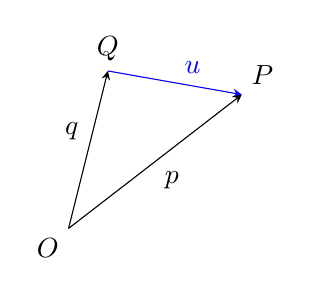
\begin{tikzpicture}
        \draw (0,0) node [anchor=north east] {$O$};
        \draw [->,>=stealth] (0,0) -- (0.5, 2) node [anchor=south] {$Q$} node [pos=0.5, anchor=south east] {$\vv{q}$};
        \draw [->,>=stealth, color=blue] (0.5,2) -- (2.2, 1.7) node [anchor=south west, color=black] {$P$} node [pos=0.5, anchor=south west] {$\vv{u}$};
        \draw [->,>=stealth] (0,0) -- (2.2, 1.7) node [pos=0.5, anchor=north west] {$\vv{p}$};
    \end{tikzpicture}
\end{center}

With this description of displacement vectors, we can define geometric objects such as lines and planes using equations involving vectors.

\subsection{Lines}

A general point on a line through $\vv{a}$ in the direction of $\vv{u} \neq \vv{0}$
can be written as
$$
\vv{r} = \vv{a} + \lambda \vv{u}, \quad \quad \lambda \in \R.
$$
This is known as the \vocab{parametric form} of the line. Note the similarity between this equation and the one for a line in the complex plane.

\begin{center}
    \begin{tikzpicture}
        \draw (0,0) node [anchor=north east] {$O$};

        \draw [dashed] (-1.5, 1.25) -- (3, 2.375);

        \draw [->,>=stealth] (0, 0) -- (-0.5, 1.5) node [anchor=north east] {$\vv{a}$};
        \draw [->, >=stealth] (-0.5, 1.5) -- (0.25, 1.6875) node [anchor=south] {$\vv{u}$};
        \draw [->, >=stealth, color=blue] (0,0) -- (2.25, 2.1875) node [anchor=north west] {$\vv{r}$};
    \end{tikzpicture}
\end{center}

To eliminate the parameter from this equation, we can take the cross product with $\vv{u}$
\begin{align*}
    \vv{u} \times \vv{r} &= \vv{u} \times (\vv{a} + \lambda \vv{u})\\
                         &= \vv{u} \times \vv{a}  \\
\implies \vv{u} \times (\vv{r} - \vv{a}) &= \vv{0}.
\end{align*}

With this in mind, consider also the related equation $\vv{u} \times \vv{r} = \vv{c}$ with $\vv{u}, \vv{c} \neq \vv{0}$. From this, $\vv{u} \cdot (\vv{u} \times \vv{r}) = \vv{u} \cdot \vv{c} = \vv{0}$, so if $\vv{u} \cdot \vv{c} \neq 0$, this is inconsistent and there is no solutions. Otherwise, if $\vv{u} \cdot \vv{c}= \vv{0}$, then $\vv{u} \times (\vv{u} \times \vv{c}) = -|\vv{u}|^2 \vv{c}$, so $\vv{a} = \frac{-1}{|\vv{u}|^2}(\vv{u} \times \vv{c})$ is one solution. Then $\vv{r} = \vv{a} + \lambda \vv{u}$ is the general solution.


\subsection{Planes}

A general point on a plane $\Pi$ thorough $\vv{a}$ with directions $\vv{u}, \vv{v}$ in the plane ($\vv{u} \not \parallel \vv{v}$) is
$$
\vv{r} = \vv{a} + \lambda \vv{u} + \mu \vv{v}, \quad \quad \lambda, \mu \in \R.
$$

\begin{center}
    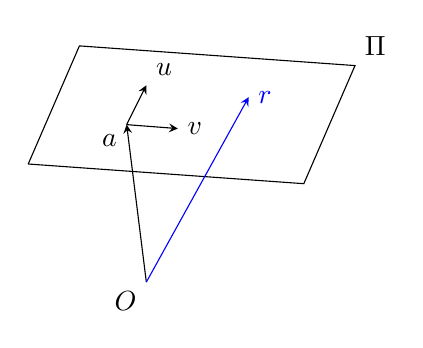
\begin{tikzpicture}
        \draw [color=black] (0, 0) -- (3.5, -0.25) -- (4.15, 1.25) -- (0.65, 1.5) -- (0,0);

        \draw (4.15, 1.25) node [color=black, anchor=south west] {$\Pi$};

        \draw (1.5,-1.5) node [anchor=north east] {$O$};

        % \draw [dashed] (-1.5, 1.25) -- (3, 2.375);

        
        \draw [->,>=stealth] (1.25, 0.5) -- (1.5, 1) node [anchor=south west] {$\vv{u}$};
        \draw [->,>=stealth] (1.25, 0.5) -- (1.9, 0.45) node [anchor=west] {$\vv{v}$};

        \draw [->,>=stealth] (1.5, -1.5) -- (1.25, 0.5) node [anchor=north east] {$\vv{a}$};

        \draw [->,>=stealth, color=blue] (1.5, -1.5) -- (2.8, 0.85) node [anchor=west] {$\vv{r}$};
    \end{tikzpicture}
\end{center}

An alternative form comes from considering a normal to the plane, $\vv{n}= \vv{u} \times \vv{v}$ ($\neq \vv{0}$). With this, we get
\begin{align*}
    \vv{n} \cdot \vv{r} &= \vv{n} \cdot \vv{a}  \\
\implies   \vv{n} \cdot (\vv{r} - \vv{a}) &= 0.
\end{align*}
For a geometric interpretation of this, note that $\vv{r} - \vv{a}$ is the displacement in the direction of the plane,and thus should be perpendicular to $\vv{n}$, a normal to the plane.

\subsection{Other Vector Equations}

To handel other vector equations, a general strategy is to manipulate equations and dot/cross with constant vectors.

\begin{example}[Vector Equation of a Sphere]
    We will attempt to find a geometric interpretation of the vector equation
    $$
    |\vv{r}|^2 + \vv{r} \cdot \vv{a} = k,
    $$
    with $\vv{a}$, $k$ constant.

    Here, we can `complete the square' to get
    $$
    \left|\vv{r} + \frac{1}{2}\vv{a}\right|^2 = k + \frac{1}{4}|\vv{a}|^2,
    $$
    which is a sphere with center $-\frac{1}{2}\vv{a}$ and radius $(k + \frac{1}{4}|\vv{a}|^2)^{1/2}$, if $k > - \frac{1}{4}|\vv{a}|^2$. If this is not the case, then there is no solutions.
\end{example}

\begin{example}[Arbitrary Vector Equation]
    We will solve the vector equation
    $$
    \vv{r} + \vv{a} \times (\vv{b} \times \vv{r}) = \vv{c},
    $$
    where $\vv{a}, \vv{b}, \vv{c}$ are given.

    We will use the `dot and cross stuff' approach. We use the vector triple product identity to rewrite this as
    \begin{equation}
        \vv{r} + (\vv{a} \cdot \vv{r}) \vv{b} - (\vv{a} \cdot \vv{b})\vv{r} = \vv{c} \tag{$\dagger$}.
    \end{equation}
    Then dotting with $\vv{a}$ we get
    \begin{align*}
        \vv{a} \cdot \vv{r} + (\vv{a} \cdot \vv{r})(\vv{b} \cdot \vv{a}) - (\vv{a} \cdot \vv{b})(\vv{a} \cdot \vv{r}) &= \vv{c} \cdot \vv{a} \nonumber \\
\implies \vv{a} \cdot \vv{r} &= \vv{c} \cdot \vv{a}. \tag{$\dagger \dagger$}
    \end{align*}
    Taking a dot product has `lost information', so we substitution $(\dagger \dagger)$ into $(\dagger)$ to get
    $$
    (1 - \vv{a} \cdot \vv{b}) \vv{r} = \vv{c} - (\vv{a} \cdot \vv{c}) \vv{b}.
    $$

    If $\vv{a} \cdot \vv{b} \neq 1$, then we can rearrange to get our solution
    $$
        \vv{r} = \frac{1}{1 - \vv{a} \cdot \vv{b}} ( \vv{c} - (\vv{a} \cdot \vv{c}) \vv{b}),
    $$
    which is a point.

    If $\vv{a} \cdot \vv{b} = 1$, then $\vv{c} - (\vv{a} \cdot \vv{c})\vv{b} \neq \vv{0}$ would cause the equation to be inconsistent. So if $\vv{c} - (\vv{a} \cdot \vv{c})\vv{b} = \vv{0}$, then $(\dagger)$ can be rewritten
    $$
    (\vv{a} \cdot \vv{r} - \vv{a} \cdot \vv{c}) \vv{b} = \vv{0},
    $$
    of which the set of solutions is given by $(\dagger \dagger)$, a plane.
\end{example}

\section{Index Notation \& The Summation Convention}

Returning to the component approach that we began to develop earlier, we will now introduce some machinery to deal with algebraically with components in an easier way.

{\color{red} This section needs to be rewritten.}

\subsection{Components, $\delta$ and $\varepsilon$}

Begin by writing vectors $\vv{a}$, $\vv{b}$, $\dots$ in terms of components $a_i, b_i$ with respect to an orthonormal, right-handed basis $\{\vv{e}_i\}$. In the following discussion, the indices $i$, $j$, $k$, $l$, $p$, $q$, $\dots$ will take on values $1, 2, 3$\footnote{This corresponds to the number of basis vectors, and the approach used will naturally generalize to indices taking on more values.}.

Using indices, we can take some vector $\vv{c} = \alpha \vv{a} + \beta \vv{b}$ and express the components as $c_i = [\alpha \vv{a} + \beta \vv{b}]_i = \alpha a_i + \beta b_i$, for $i = 1, 2, 3$ (a \vocab{free variable}). Using the same notation, we can write things like
$$
\vv{a} \cdot \vv{b} = \sum_i a_i b_i,
$$
and
\begin{align*}
    \vv{x} &= \vv{a} + (\vv{b} \cdot \vv{c}) \vv{d} \\
\iff x_j &= a_j + \left(\sum_k b_k c_k\right) d_j, \quad \quad \text{for }j = 1, 2, 3.
\end{align*}

\begin{definition}[Kronecker Delta Symbol]
    We define the \vocab{Kronecker delta} symbol to be
    $$
    \delta_{ij} = \begin{cases}
        1 &\mbox{if } i = j, \\
        0 &\mbox{if } i \neq j.
       \end{cases}
    $$
\end{definition}

With this definition, we get $\vv{e}_i \cdot \vv{e}_j = \delta_{ij}$, which encodes our orthonormality condition from before. Then
\begin{align*}
    \vv{a} \cdot \vv{b} &= \left(\sum_i a_i \vv{e}_i\right)\left(\sum_i b_j \vv{e}_j\right) \\
    &= \sum_{ij} a_i b_j \vv{e}_i \cdot \vv{e}_j \\
    &= \sum_{ij} a_i b_j \delta_{ij} \\
    &= \sum_i a_i b_i.
\end{align*}

\begin{definition}[Levi-Civita Symbol]
    We define the \vocab{Levi-Civita symbol} such that
    $$
    \varepsilon_{ijk} = \begin{cases}
        +1 &\mbox{if } (i\ j\ k) \text{ is an even permutation of } (1\ 2\ 3), \\
        -1 &\mbox{if } (i\ j\ k) \text{ is an odd permutation of } (1\ 2\ 3), \\ 
        0 &\mbox{otherwise}
       \end{cases}
    $$
\end{definition}

For example,
\begin{align*}
    \varepsilon_{123} =  \varepsilon_{231} =  \varepsilon_{312} = +1, \\
    \varepsilon_{321} =  \varepsilon_{213} =  \varepsilon_{132} = -1, \\
    \varepsilon_{ijk} = 0 \text{ if any of } i,j,k \text{ repeat.}
\end{align*}

The Levi-Civita symbol is \vocab{totally antisymetric}, in that exchangin a pair of indices produces a change in sign.

With this definition, in our right-handed orthonormal basis we have
$$
\vv{e}_i \times \vv{e}_j = \sum_k \varepsilon_{ijk} \vv{e}_k,
$$
for example
$$
\vv{e}_2 \times \vv{e}_1 = \sum_k \varepsilon_{21k}\vv{e}_k = \varepsilon_{213} \vv{e}_3 = - \vv{e}_3.
$$

So we can compute the cross product of two vectors as
\begin{align*}
    \vv{a}\times \vv{b} &= \left(\sum_i a_i \vv{e}_i\right) \times \left(\sum_j b_j \vv{e}_j\right) \\
    &= \sum_{ij} a_i b_j \vv{e}_i \times \vv{e}_j \\
    &= \sum_{ijk} a_i b_j \varepsilon_{ijk} \vv{e}_k \\
\iff (\vv{a} \times \vv{b})_k = \sum_{ij} \varepsilon_{ijk} a_i b_j.
\end{align*}

For example, $(\vv{a} \times \vv{b})_3 = \sum_{ij} \varepsilon_{ij3} a_i b_j = \varepsilon_{123} a_1 b_2 + \varepsilon_{213} a_2 b_1 = a_1 b_2 - a_2 b_1$, as we had before.

\subsection{Summation Convention}

With components and index notation, indices that appear twice in a given term are usually summed over. In the \vocab{summation convention}, we omit the sigma ($\sum$) signs for repeated indices, and the sums are implicitly understood.

\begin{example}[Examples of the Summation Convention]
    The following all use the summation convention.
    \begin{enumerate}[label=(\roman*)]
        \item $a_i \delta_{ij} = a_1 \delta_{1j} + a_2 \delta_{2j} + a_3\delta_{3j} = a_j$.
        \item $\vv{a} \cdot \vv{b} = a_i b_i$.
        \item $(\vv{a} \times \vv{b})_i= \varepsilon_{ijk}a_j b_k$.
        \item $\vv{a} \cdot (\vv{b} \times \vv{c}) = \varepsilon_{ijk} a_i b_j c_k$.
        \item $\delta_{ii} = \delta_{11} + \delta_{22} + \delta_{33} = 3$.
        \item $[(\vv{a} \cdot \vv{c})\vv{b} - (\vv{a} \cdot \vv{b})\vv{c}]_i = (\vv{a} \cdot \vv{c})b_i + (\vv{a} \cdot \vv{b})c_i = a_j c_j b_i - a_k b_k c_i$.
    \end{enumerate}
\end{example}

We can explicitly define the rules of the summation convention as follows.

\begin{definition}[Summation Convention Rules]
    When using the summation convention, we have the following rules.
    \begin{enumerate}[label=(\roman*)]
        \item An index occurring exactly once in any given term must appear once in every term of an equation, and it can take any value -- a \vocab{free index}.
        \item Any index occurring exactly \emph{twice} in a given term is summed over -- a \vocab{repeated}, \vocab{contracted} or \vocab{dummy index}.
        \item No index can occur more than twice in a given term.
    \end{enumerate}
\end{definition}

Let's have a look at applying the summation convention to prove the vector triple product identity we stated earlier.

\begin{proposition}[Vector Triple Product Identity]
    For vectors $\vv{a}, \vv{b}, \vv{c}$, we have
    $$
    \vv{a} \times(\vv{b} \times \vv{c})=(\vv{a} \cdot \vv{c}) \vv{b}-(\vv{a} \cdot \vv{b}) \vv{c}.
    $$
\end{proposition}
\begin{proof}
We have
\begin{align*}
    [\vv{a} \times (\vv{b} \times \vv{c})]_i &= \varepsilon_{ijk} a_j (\vv{b} \times \vv{c})_k \\
        &= \varepsilon_{ijk} a_j \varepsilon_{kpq} b_p c_q \\
 &= (\varepsilon_{ijk}\varepsilon_{pqk}) a_j b_p c_q,
\end{align*}    
now $\varepsilon_{ijk}\varepsilon_{pqk} = \delta_{ip} \delta_{jq} - \delta_{iq} \delta_{jp}$ (we will prove this later on), hence
\begin{align*}
    [\vv{a} \times (\vv{b} \times \vv{c})]_i &= (\delta_{ip} \delta_{jq})a_j b_p c_q - (\delta_{iq} \delta_{jp}) a_j b_p c_q \\
    &= [(\vv{a} \cdot \vv{c})\vv{b} - (\vv{a} \cdot \vv{b})\vv{c}]_i,
\end{align*}
as required.
\end{proof}

\subsection{$\varepsilon \varepsilon$ Identities}

We will finish this section by looking at $\varepsilon \varepsilon$ identities, which can be used in various computations involving $\delta$ and $\varepsilon$ symbols.

\begin{itemize}
    \item $\varepsilon_{ijk}\varepsilon_{pqk} = \delta_{ip} \delta_{jk} - \delta_{iq} \delta_{jp} = \varepsilon_{kij} \varepsilon_{kpq}$.
    
    To check this, note that RHS and LHS are antisymmetric under $i \leftrightarrow j$, $p \leftrightarrow q$, so both vanish if $i$ \& $j$ or $p$ \& $q$ take the same value. Now it suffices to check examples $i = p = 1$, $j = q = 2$, where LHS and RHS are both $+1$, or $i = q = 1$, $j = p = 2$, where LHS and RHS are both $-1$. All other index choices giving non-zero results work similarity.

    \item $\varepsilon_{ijk} \varepsilon_{pjk} = 2 \delta_{ip}$.
    
    This comes from the above identity, where the LHS becomes $\delta_{ip} \delta_{jj} - \delta_{ij} \delta_{jp} = 3\delta_{ip} - \delta_{ip} = 2\delta_{ip}$.

    \item $\varepsilon_{ijk} \varepsilon_{ijk} = 6$.

    This follows directly from the previous result, with $i = p$. Then $2 \delta_{ii} = 6$.
\end{itemize}

% \section{Index Notation \& The Summation Convention}

